\documentclass[11pt,a4paper]{report}
\usepackage[latin1]{inputenc}
\usepackage[T1]{fontenc}  
\usepackage[french]{babel}
\usepackage{url}
\usepackage{graphicx}
\usepackage{fancyhdr}
\pagestyle{fancy}



\title{Rapport de Projet: Le voyageur de commerce}
\author{Benjamin Saint-Sever, Caitlin Dagg, Manon Pintault }
\date{\today}

\renewcommand{\headrulewidth}{1pt}
%\fancyhead[C]{\textbf{page \thepage}} 
%\fancyhead[L]{\leftmark}
\fancyhead[R]{Rapport de Projet: Le voyageur de commerce}


\renewcommand{\footrulewidth}{1pt}
%\fancyfoot[C]{\textbf{page \thepage}} 
%\fancyfoot[L]{Rapport de Projet: Le voyageur de commerce}
%\fancyfoot[R]{\leftmark}

\begin{document}

\maketitle

\tableofcontents





\chapter{Introduction}
Le but de ce projet est de fournir un programme fonctionnant en ligne de commande permettant de calculer des solutions (pas forc�ment optimales) au probl�me du voyageur de commerce m�trique (c?est-�-dire calculer le meilleur trajet � parcourir pour un ensemble de villes donn�es sans repasser par un ville d�j� visit�e). Dans le cadre de ce projet, l?ensemble des villes est donn�e sous forme de matrice de distance.

\chapter {Vie du projet}
\section{Logiciel de gestion de version}
Afin de pouvoir r�alis� ce projet, nous avons choisi d?utiliser un d�p�t en ligne : Github. Si nous avons opt� pour cette solution c?est car il nous permettait de choisir entre l?utilisation de svn ou git. De plus c?est un outil simple d?utilisation et accessible avec une simple connexion internet depuis n?importe quel support (mac, windows, linux).

\section{organisation}
Pendant toute la dur�e du projet, nous nous sommes partag� les t�ches chaque semaine. Par exemple, certains travaillaient un algorithme, l?autre s?occupait du makefile, de r�fl�chir sur le prochain algorithme � faire et le dernier cr�ait des tests et g�rait l?organisation des fichiers. Mais g�n�ralement nous rajoutions chacun des lignes de codes au diff�rents algorithmes pour am�liorer ceux-ci et r�gler quelques soucis rencontr�s . 


\chapter {Pr�sentation des algorithmes}
\section{Nearest Neighbour}


\begin{figure}[h!]
  \centering 
  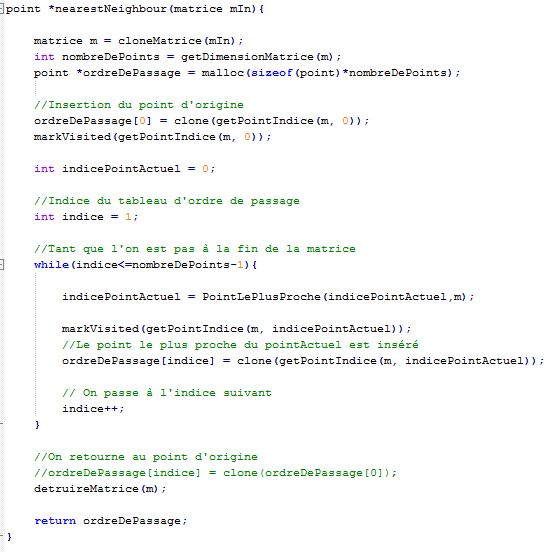
\includegraphics[height=10cm]{Nearest.JPG}
  \caption{Une heuristique simple}
\end{figure}
\newpage

\section{Prim}


\begin{figure}[h!]
  \centering 
  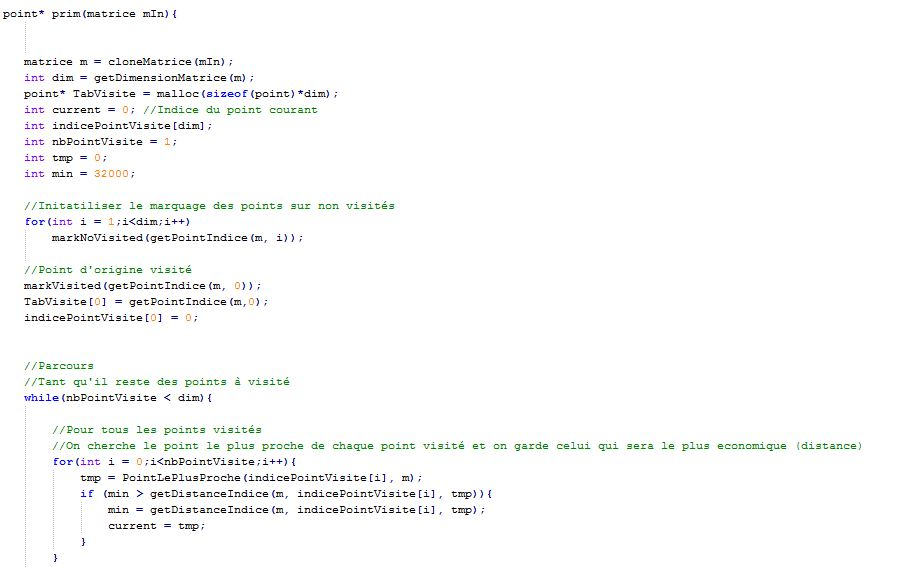
\includegraphics[height=10cm]{Prim_part1.JPG}
  \caption{Un algorithme d'approximation}
\end{figure}

\begin{figure}[h!]
  \centering 
  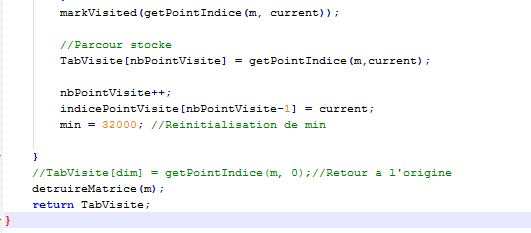
\includegraphics[height=10cm]{Prim_part2.JPG}
\end{figure}

\newpage
\section{Brute Force}


\begin{figure}[h!]
  \centering 
  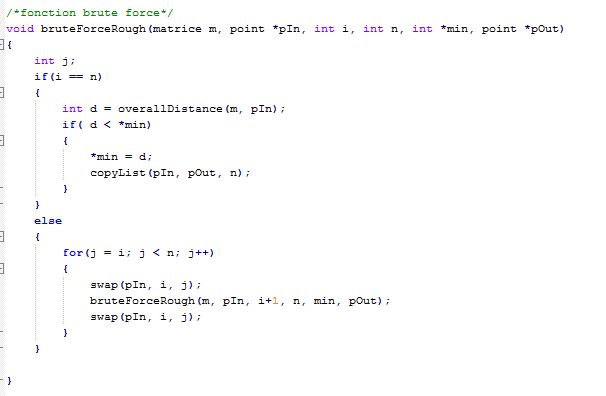
\includegraphics[height=6cm]{BF_1.JPG}
  \caption{Un algorithme exact par recherche exhaustive}
\end{figure}

\begin{figure}[h!]
  \centering 
  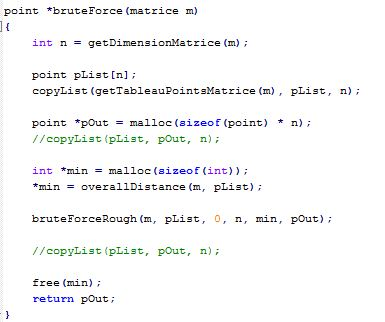
\includegraphics[height=10cm]{BF_2.JPG}
  \caption{Un algorithme exact par recherche exhaustive}
\end{figure}

\newpage
\section{Branch and Bound}


\chapter {Conclusion}






\end{document}